\subsection{External interface requirements}
\subsubsection{User interfaces}
There are two categories of users that have different interface requirements:
\begin{itemize}
	\item {\bfseries Customers}\\
	Customers belong to all demographics so a user friendly interface is needed. The customer is presented with a main menu which allows him/her to:
	\begin{itemize}
		\item line up immediately (immediate reservation) at a specific store
		\item book a visit (future reservation) at a specific store
		\item view and delete existing reservations
	\end{itemize}
	The customer will receive a notification when it is time for him/her to depart to reach the shop.\\\\
	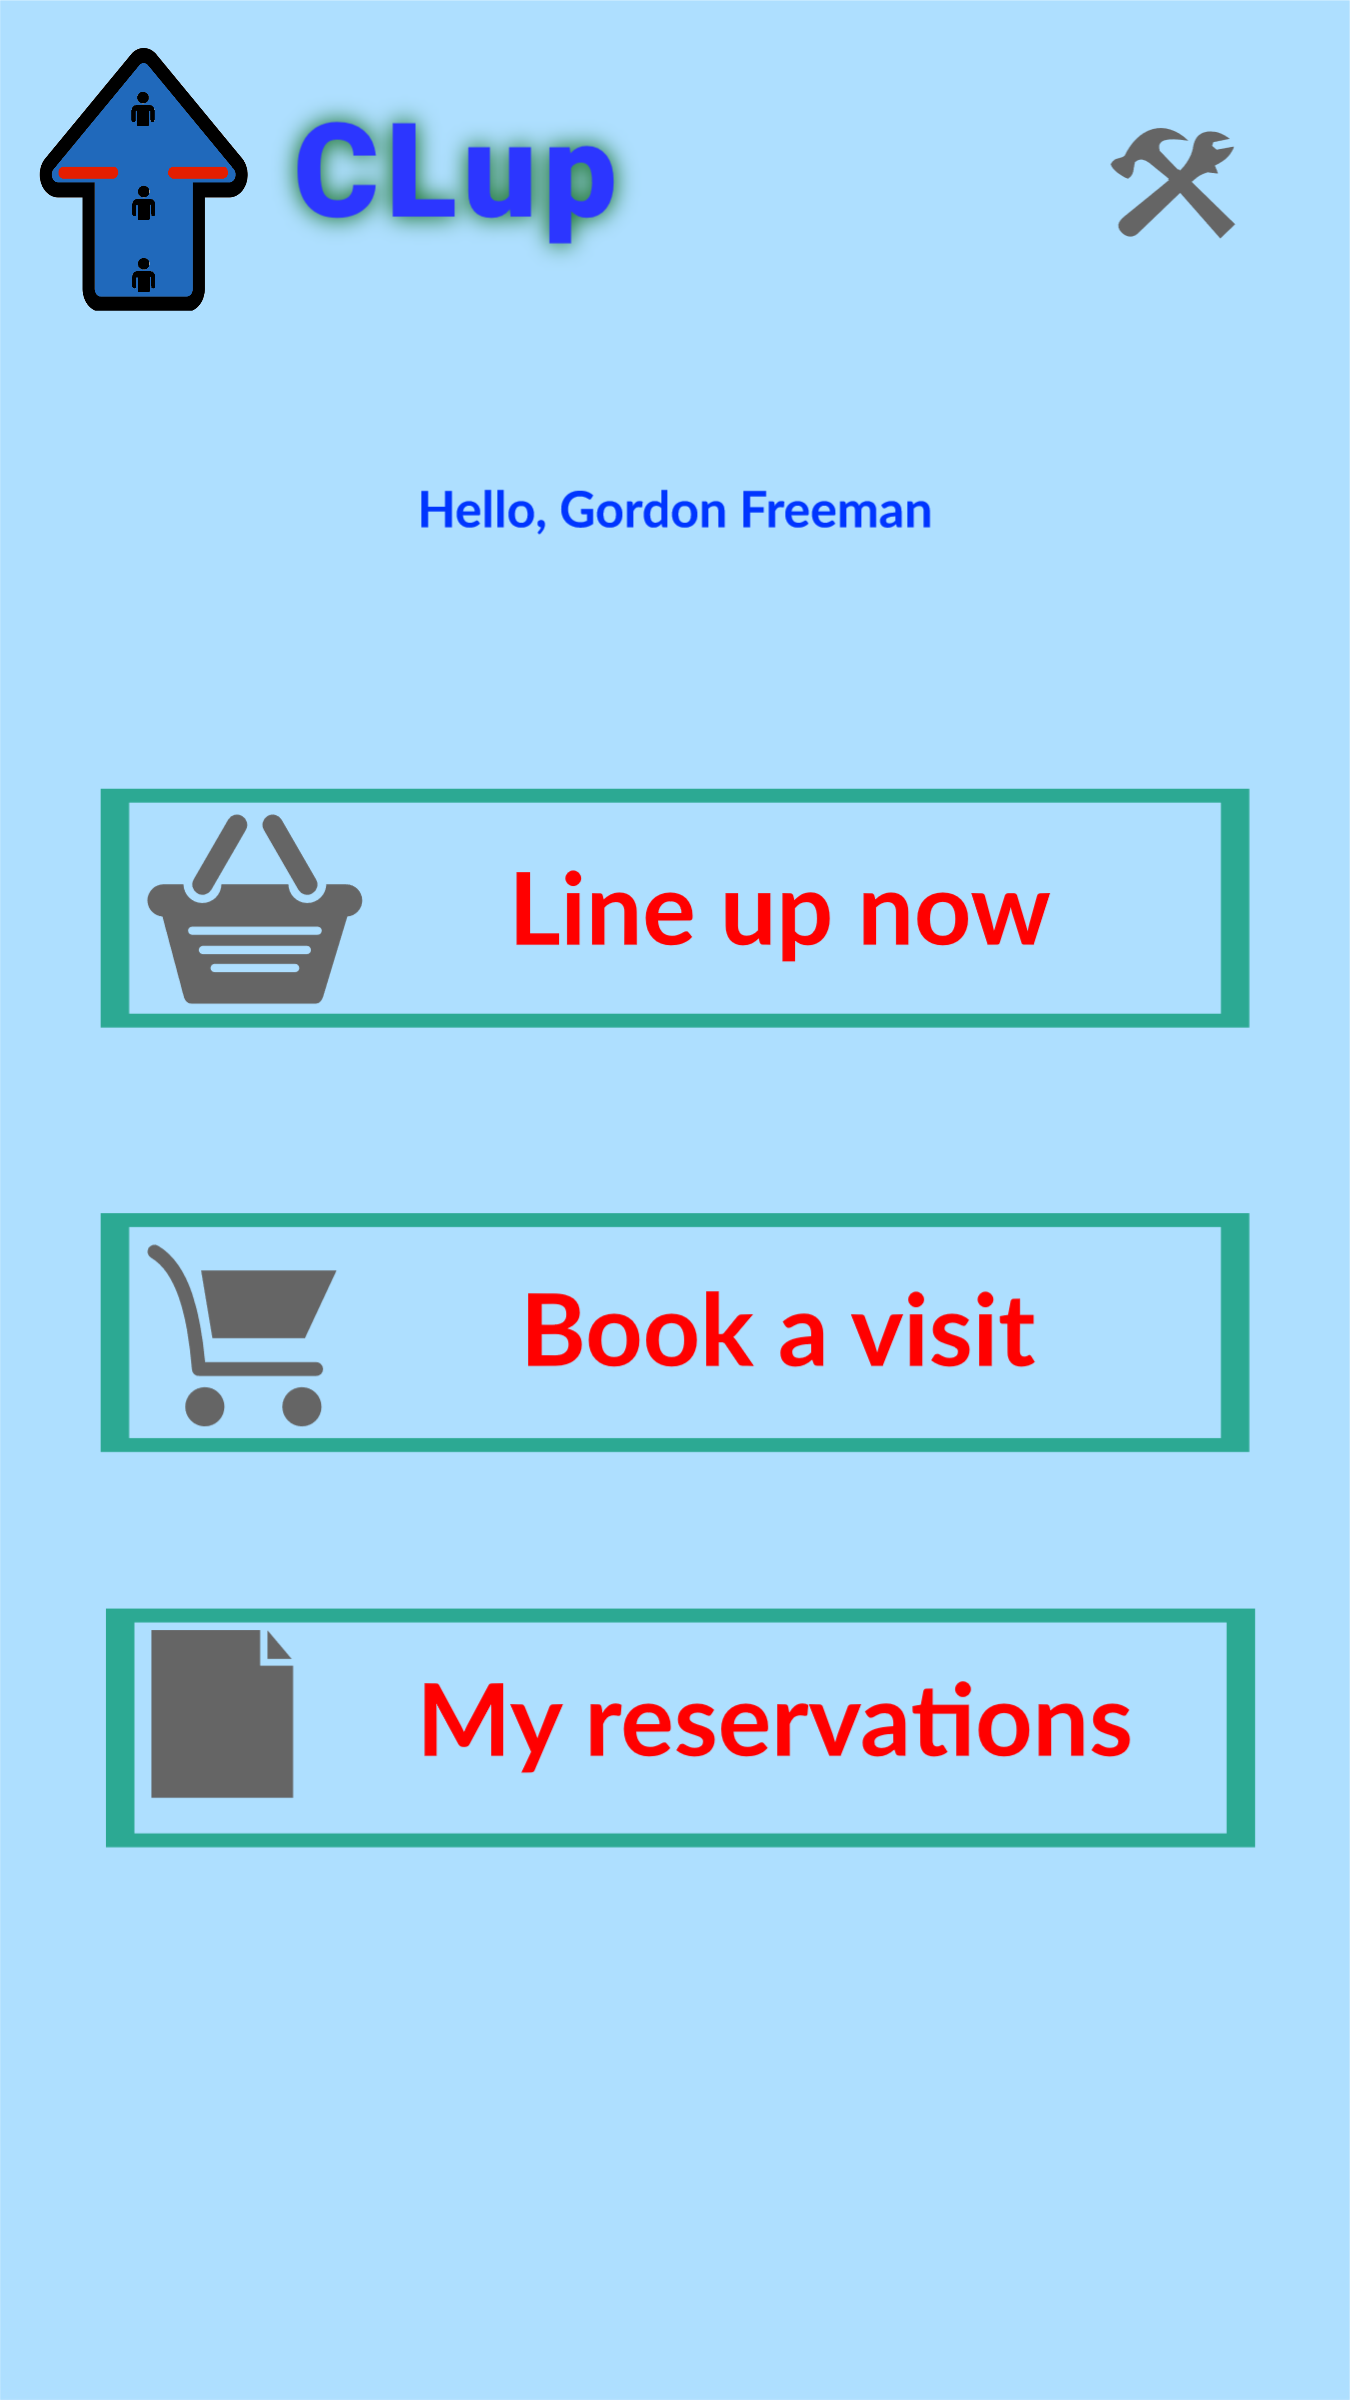
\includegraphics[scale=0.1]{Images/MainMenuCustomer.png}
	\qquad
	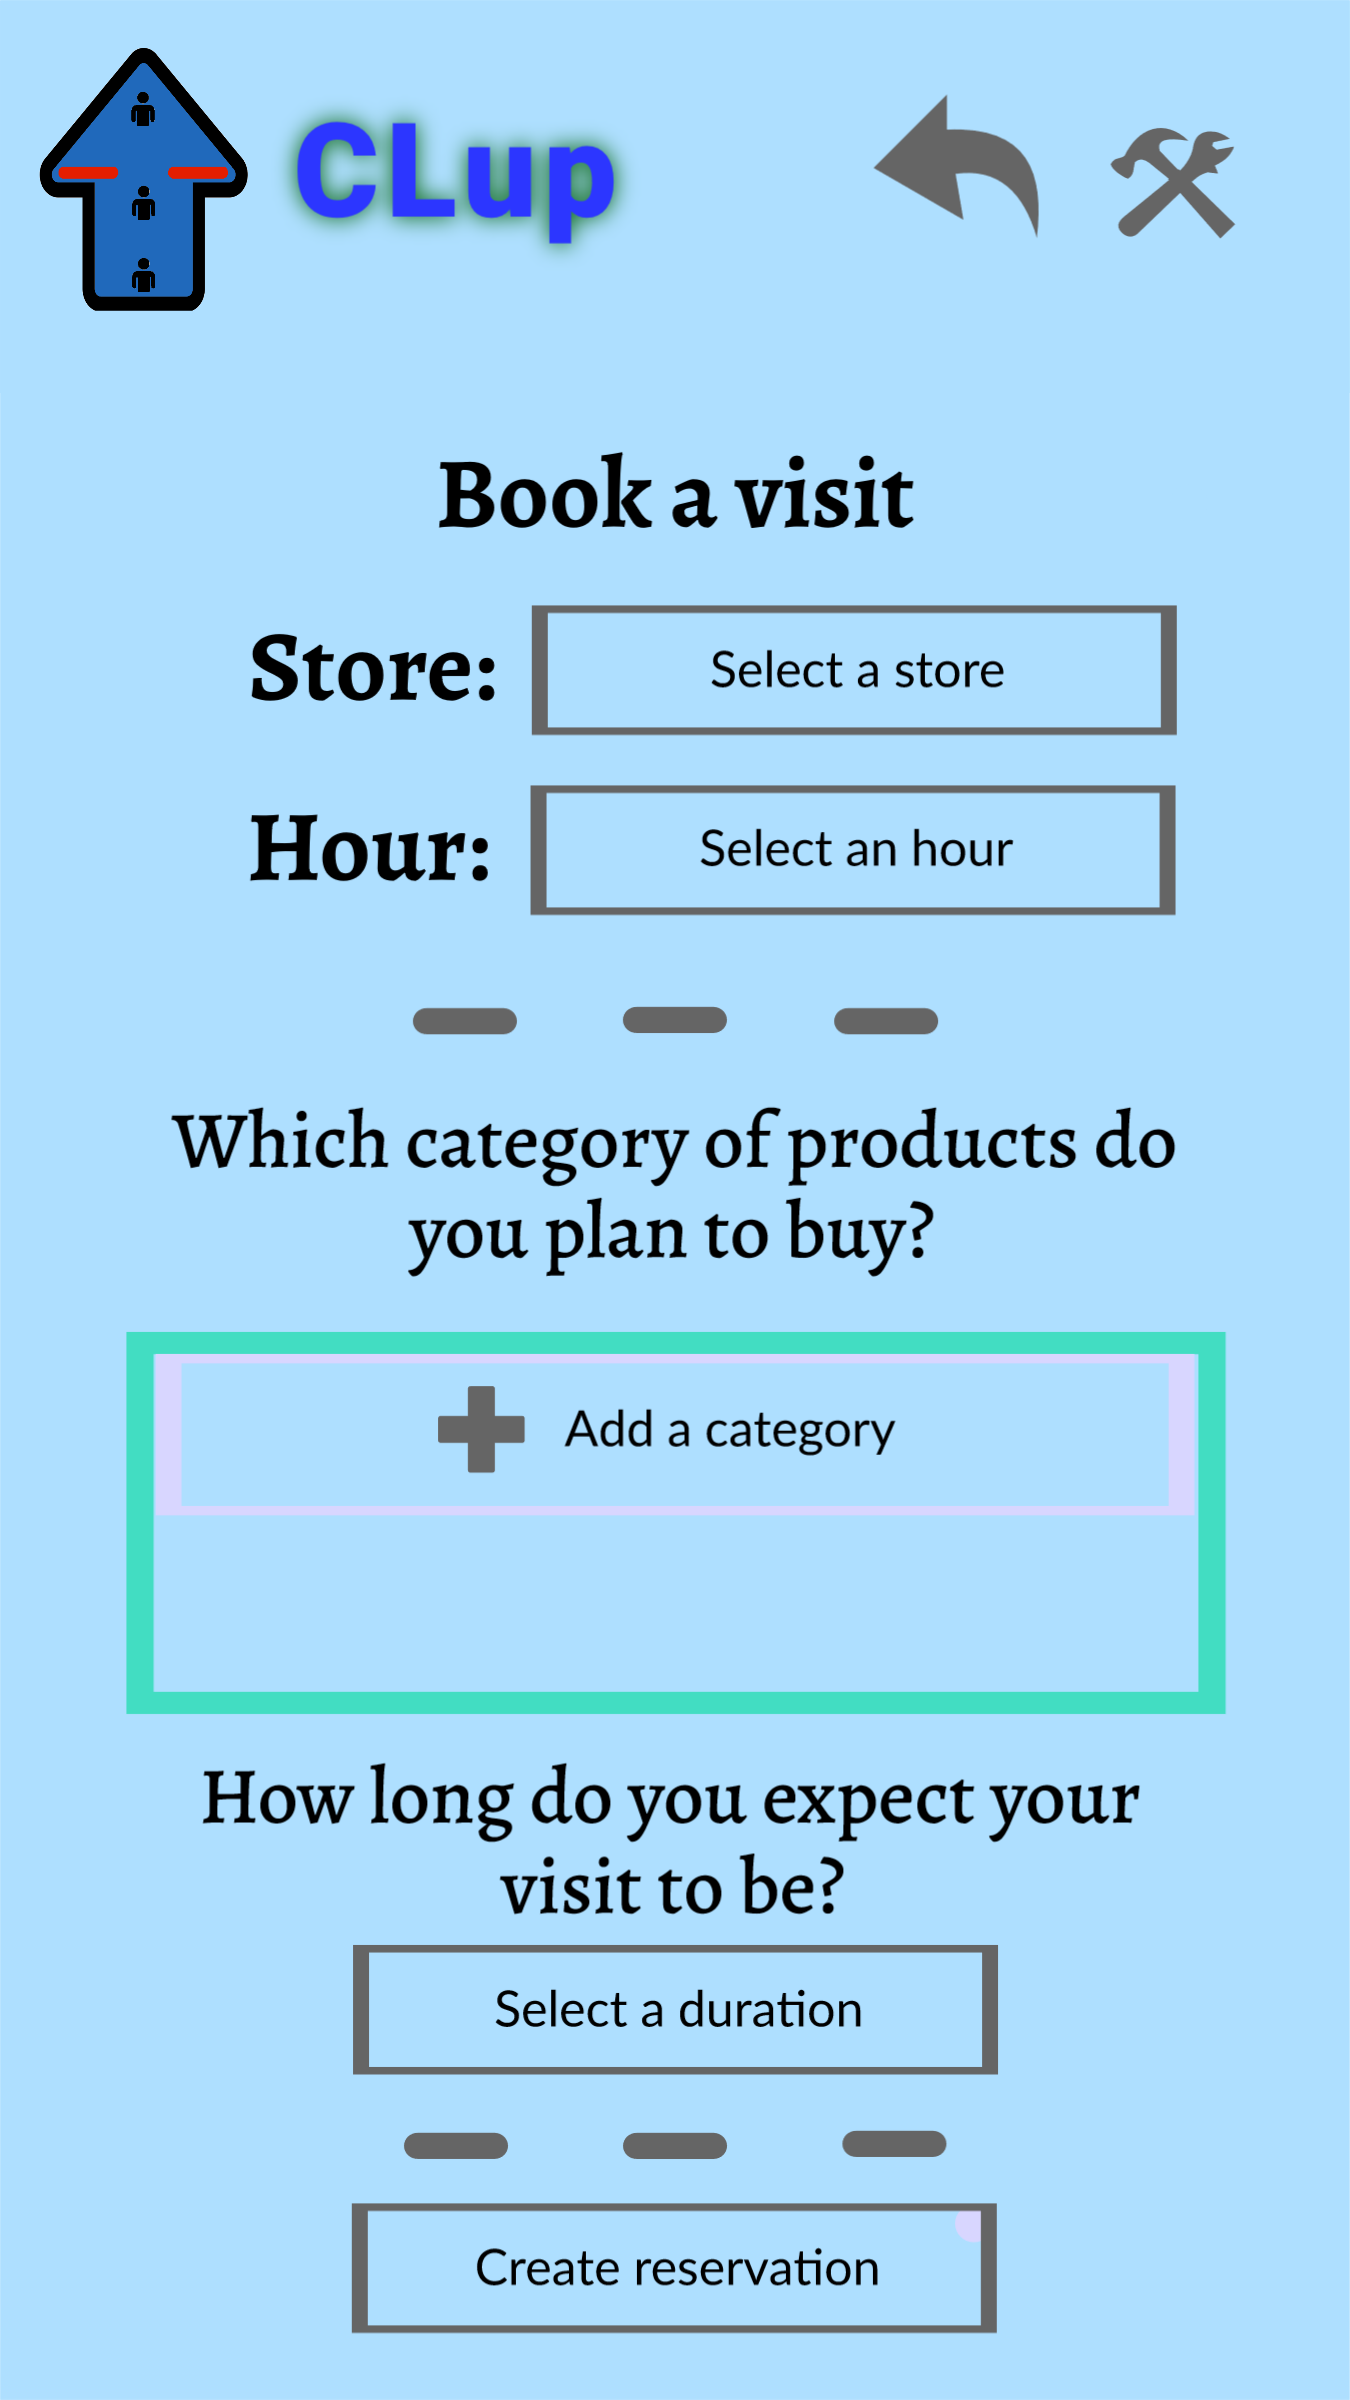
\includegraphics[scale=0.1]{Images/BookAVisit.png}
	%TODO add by car/on foot icons
	\qquad
	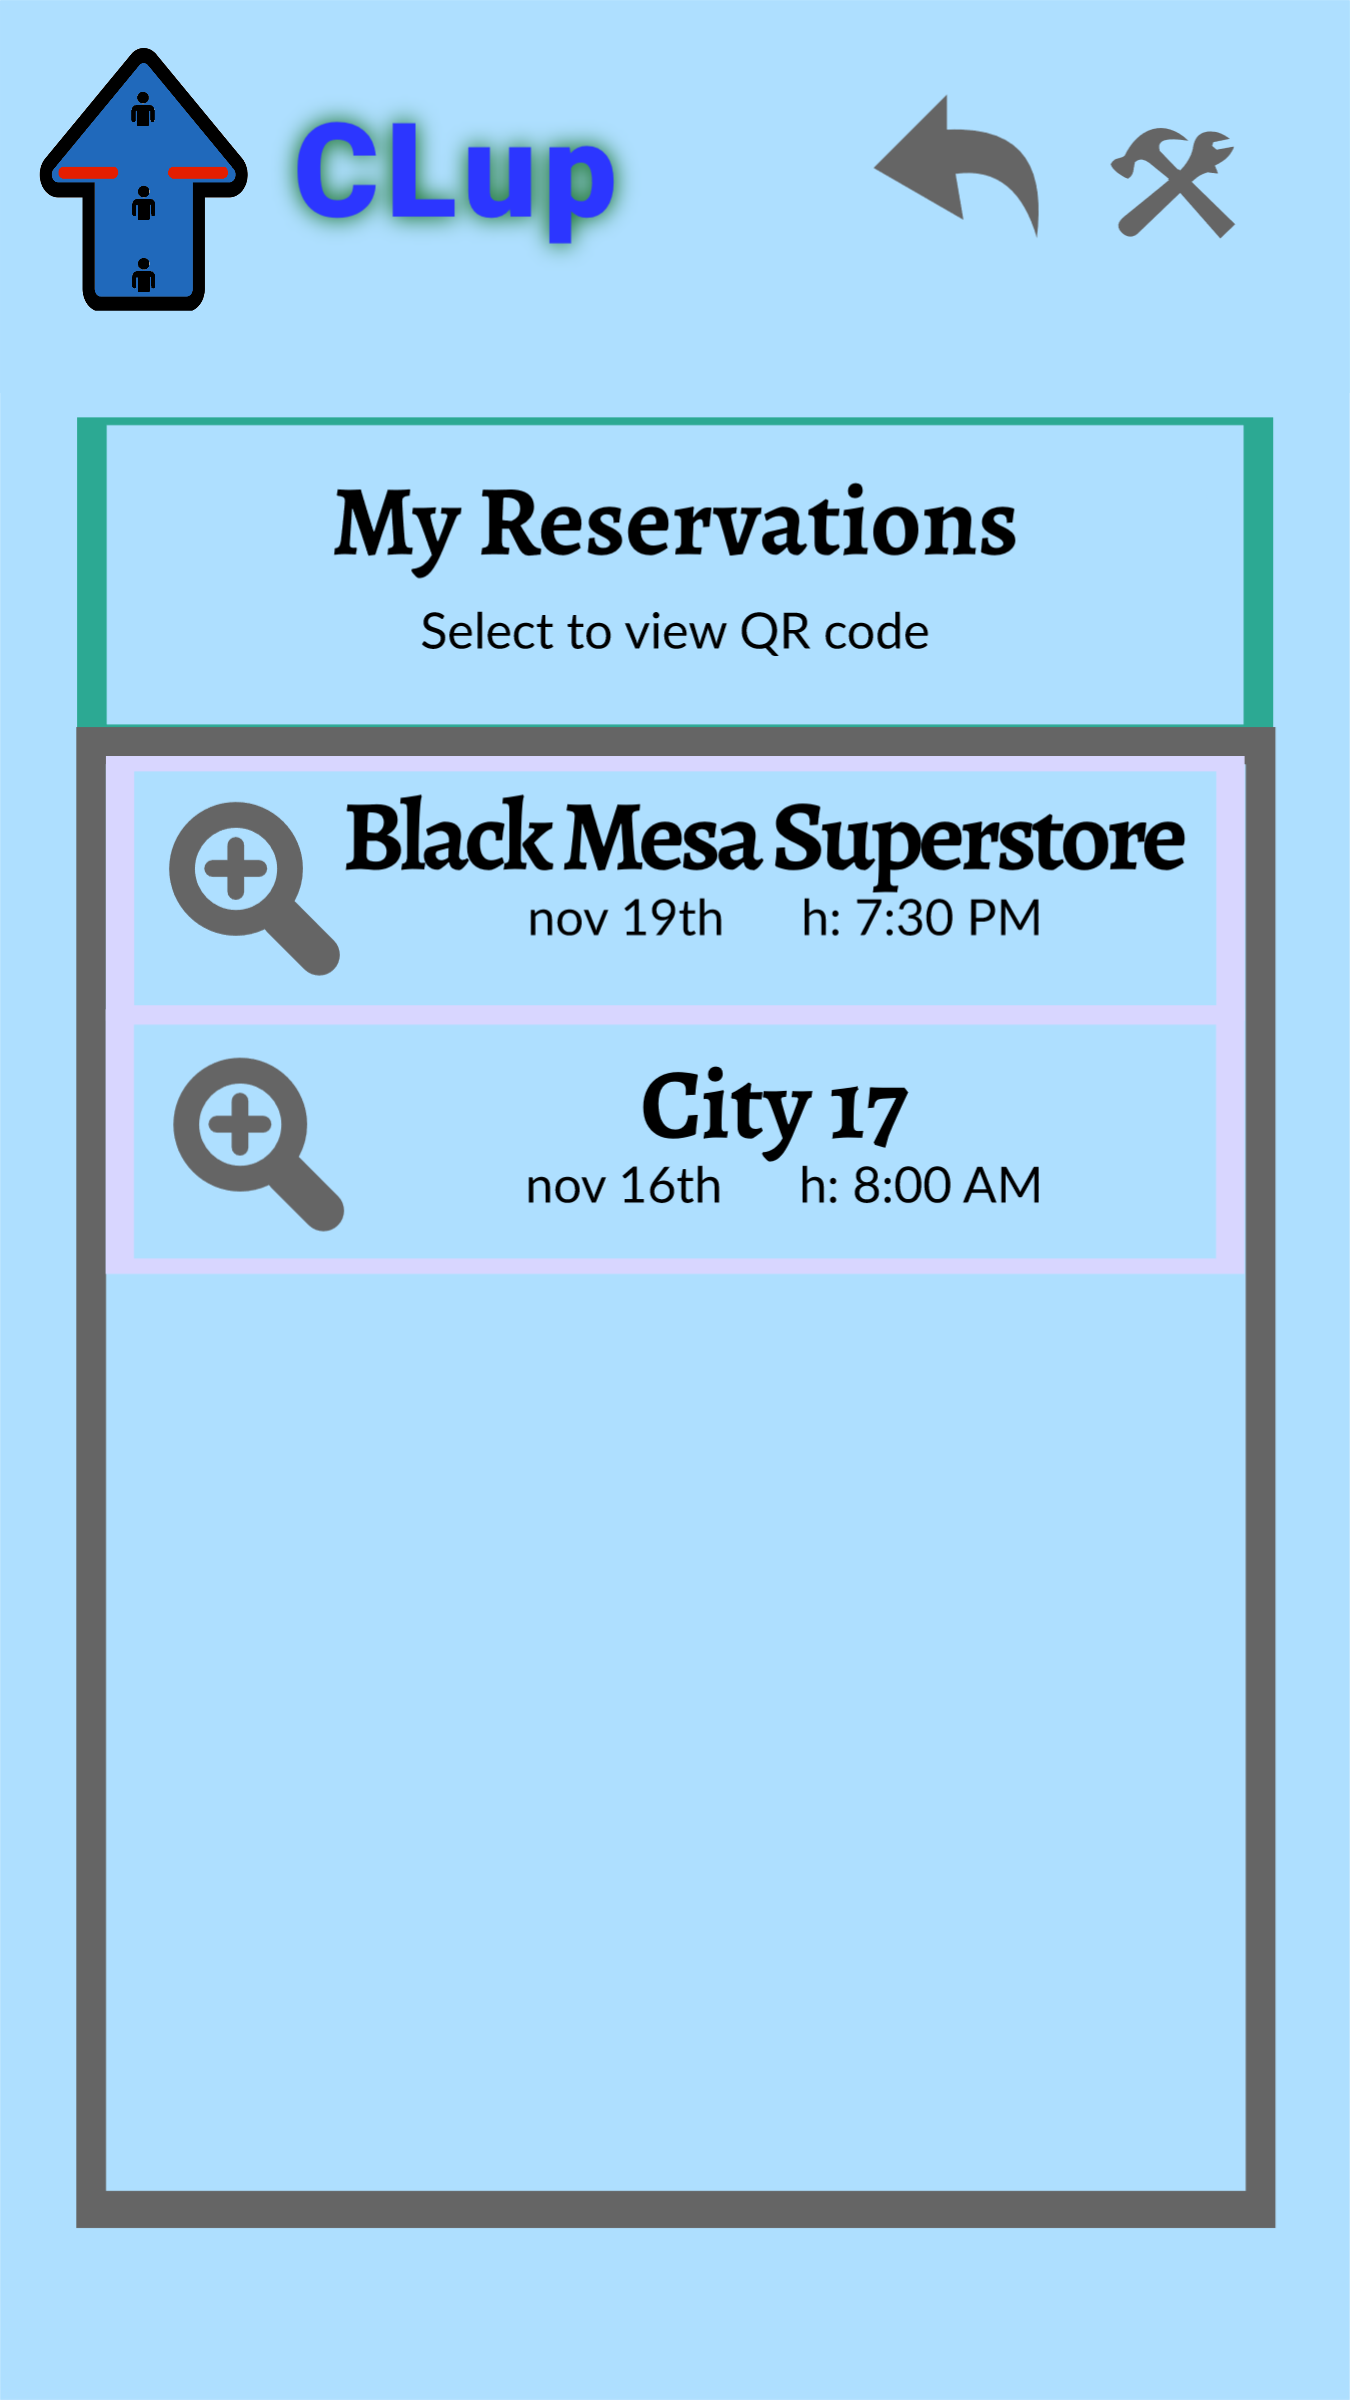
\includegraphics[scale=0.1]{Images/ShowReservations.png}
	\item {\bfseries Store owners}\\
	The store owner is presented with a main menu from which he/she can:
		\begin{itemize}
		\item register a store to the system
		\item delete a store from the system
		\item view and edit occupation for currently registered stores
	\end{itemize}
	\begin{figure}[!htb]
		\centering
		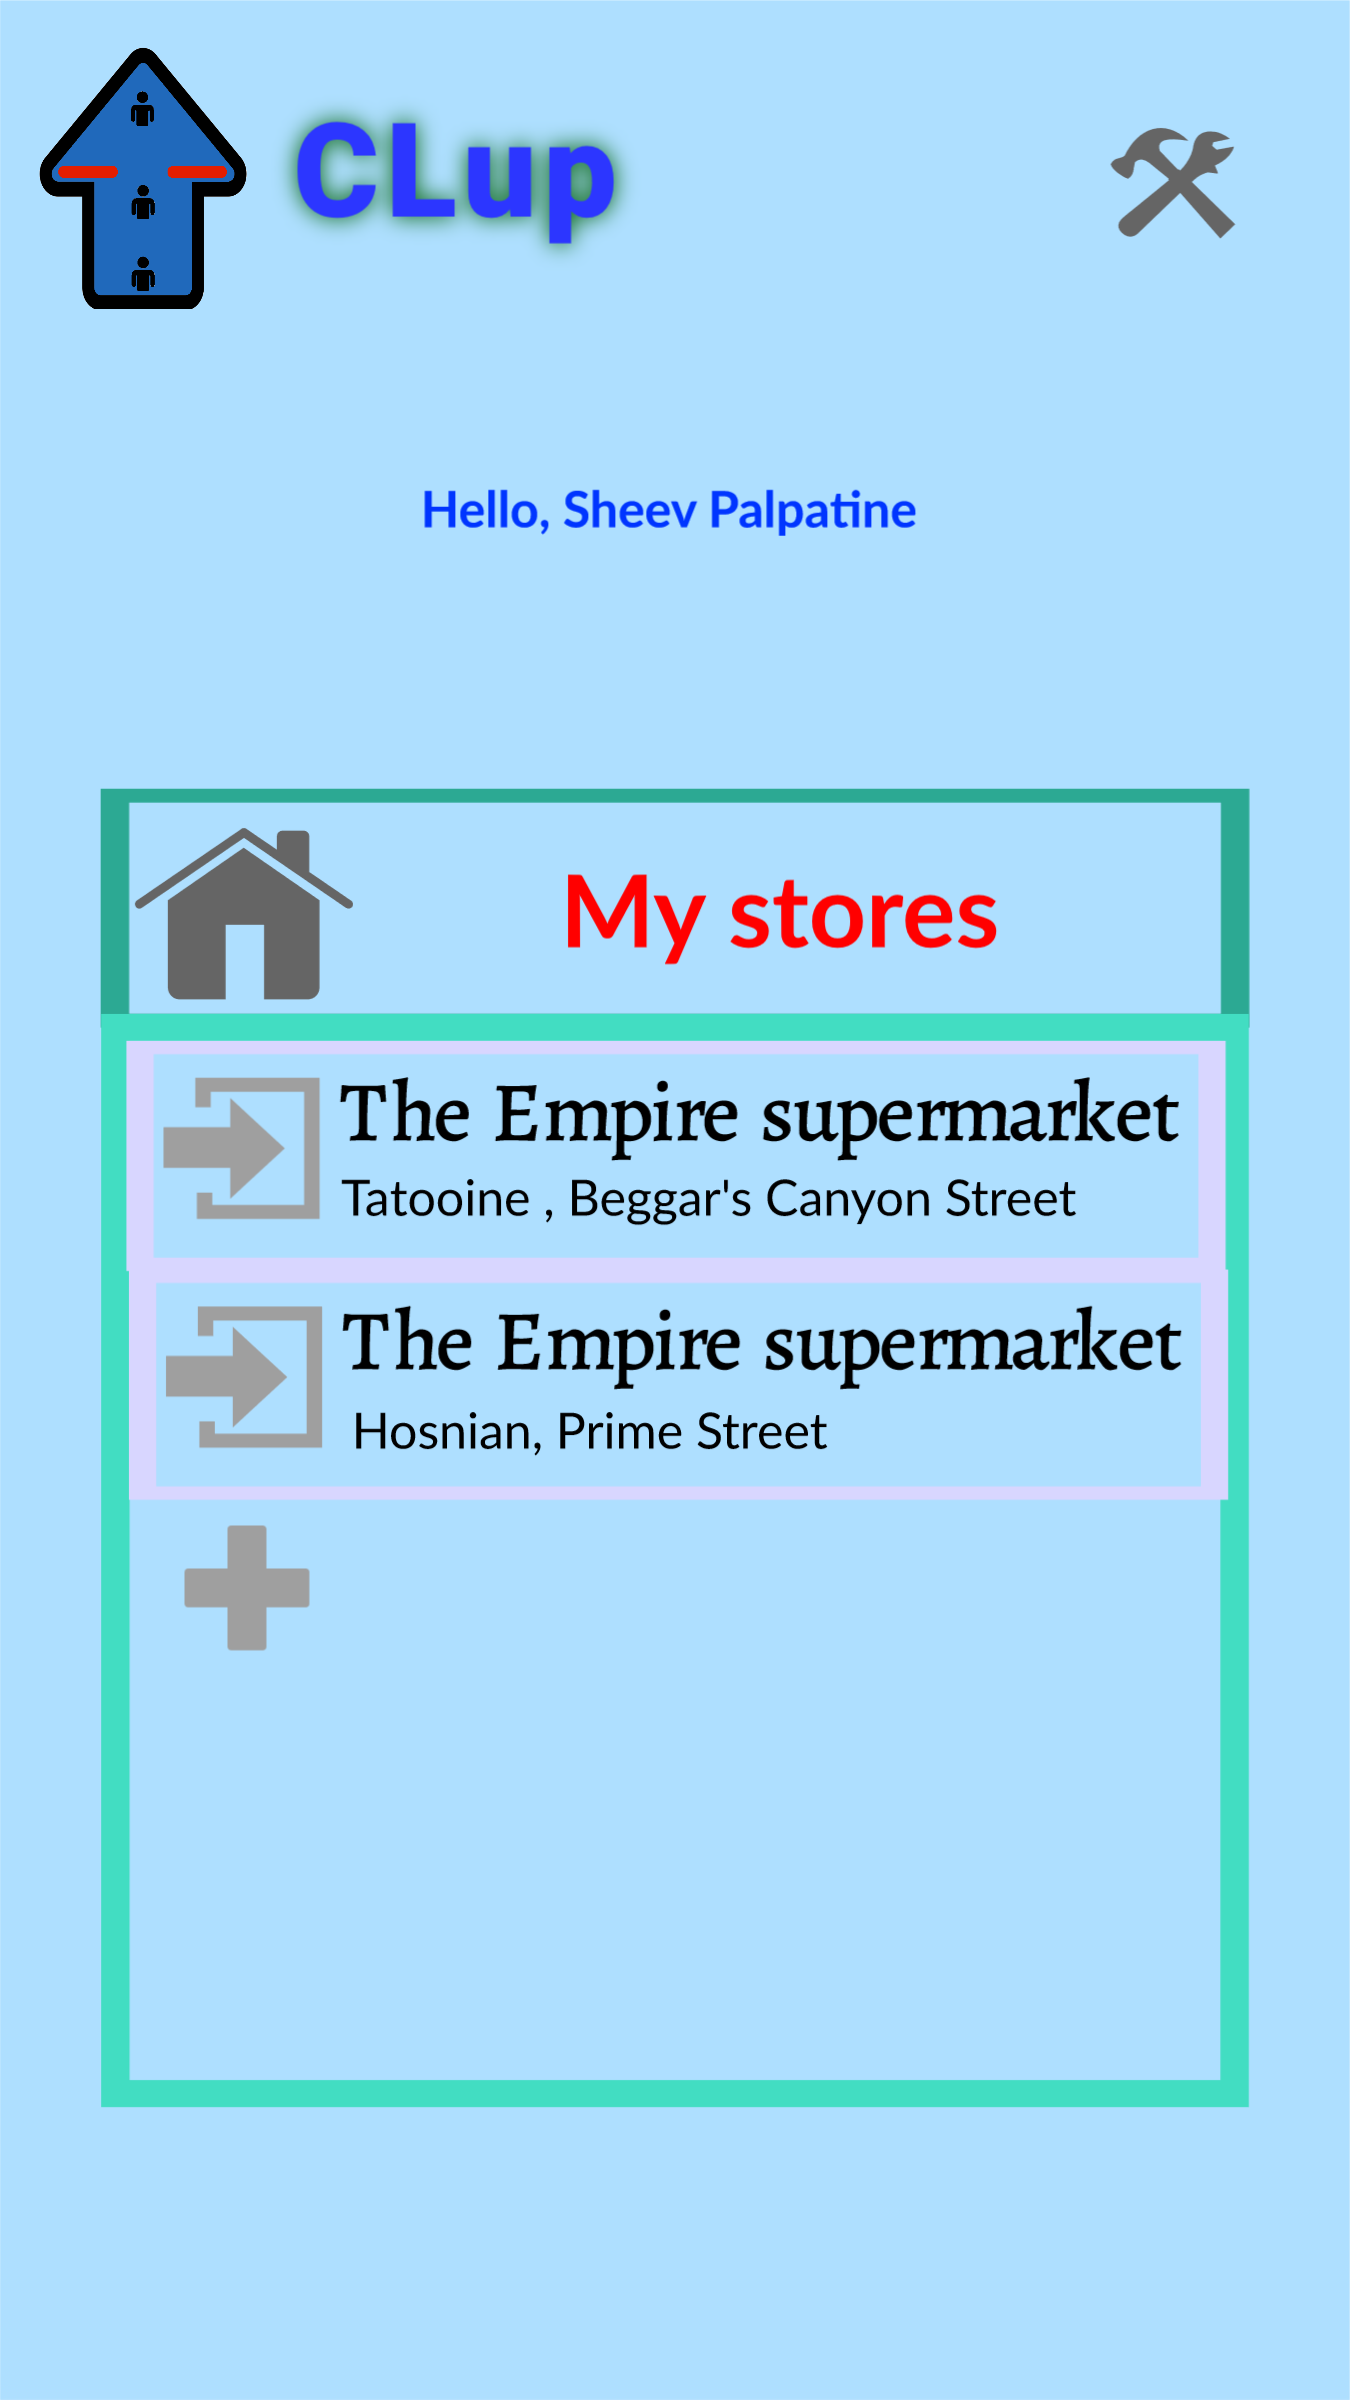
\includegraphics[scale=0.1]{Images/MainMenuOwner.png}
		\qquad \qquad
		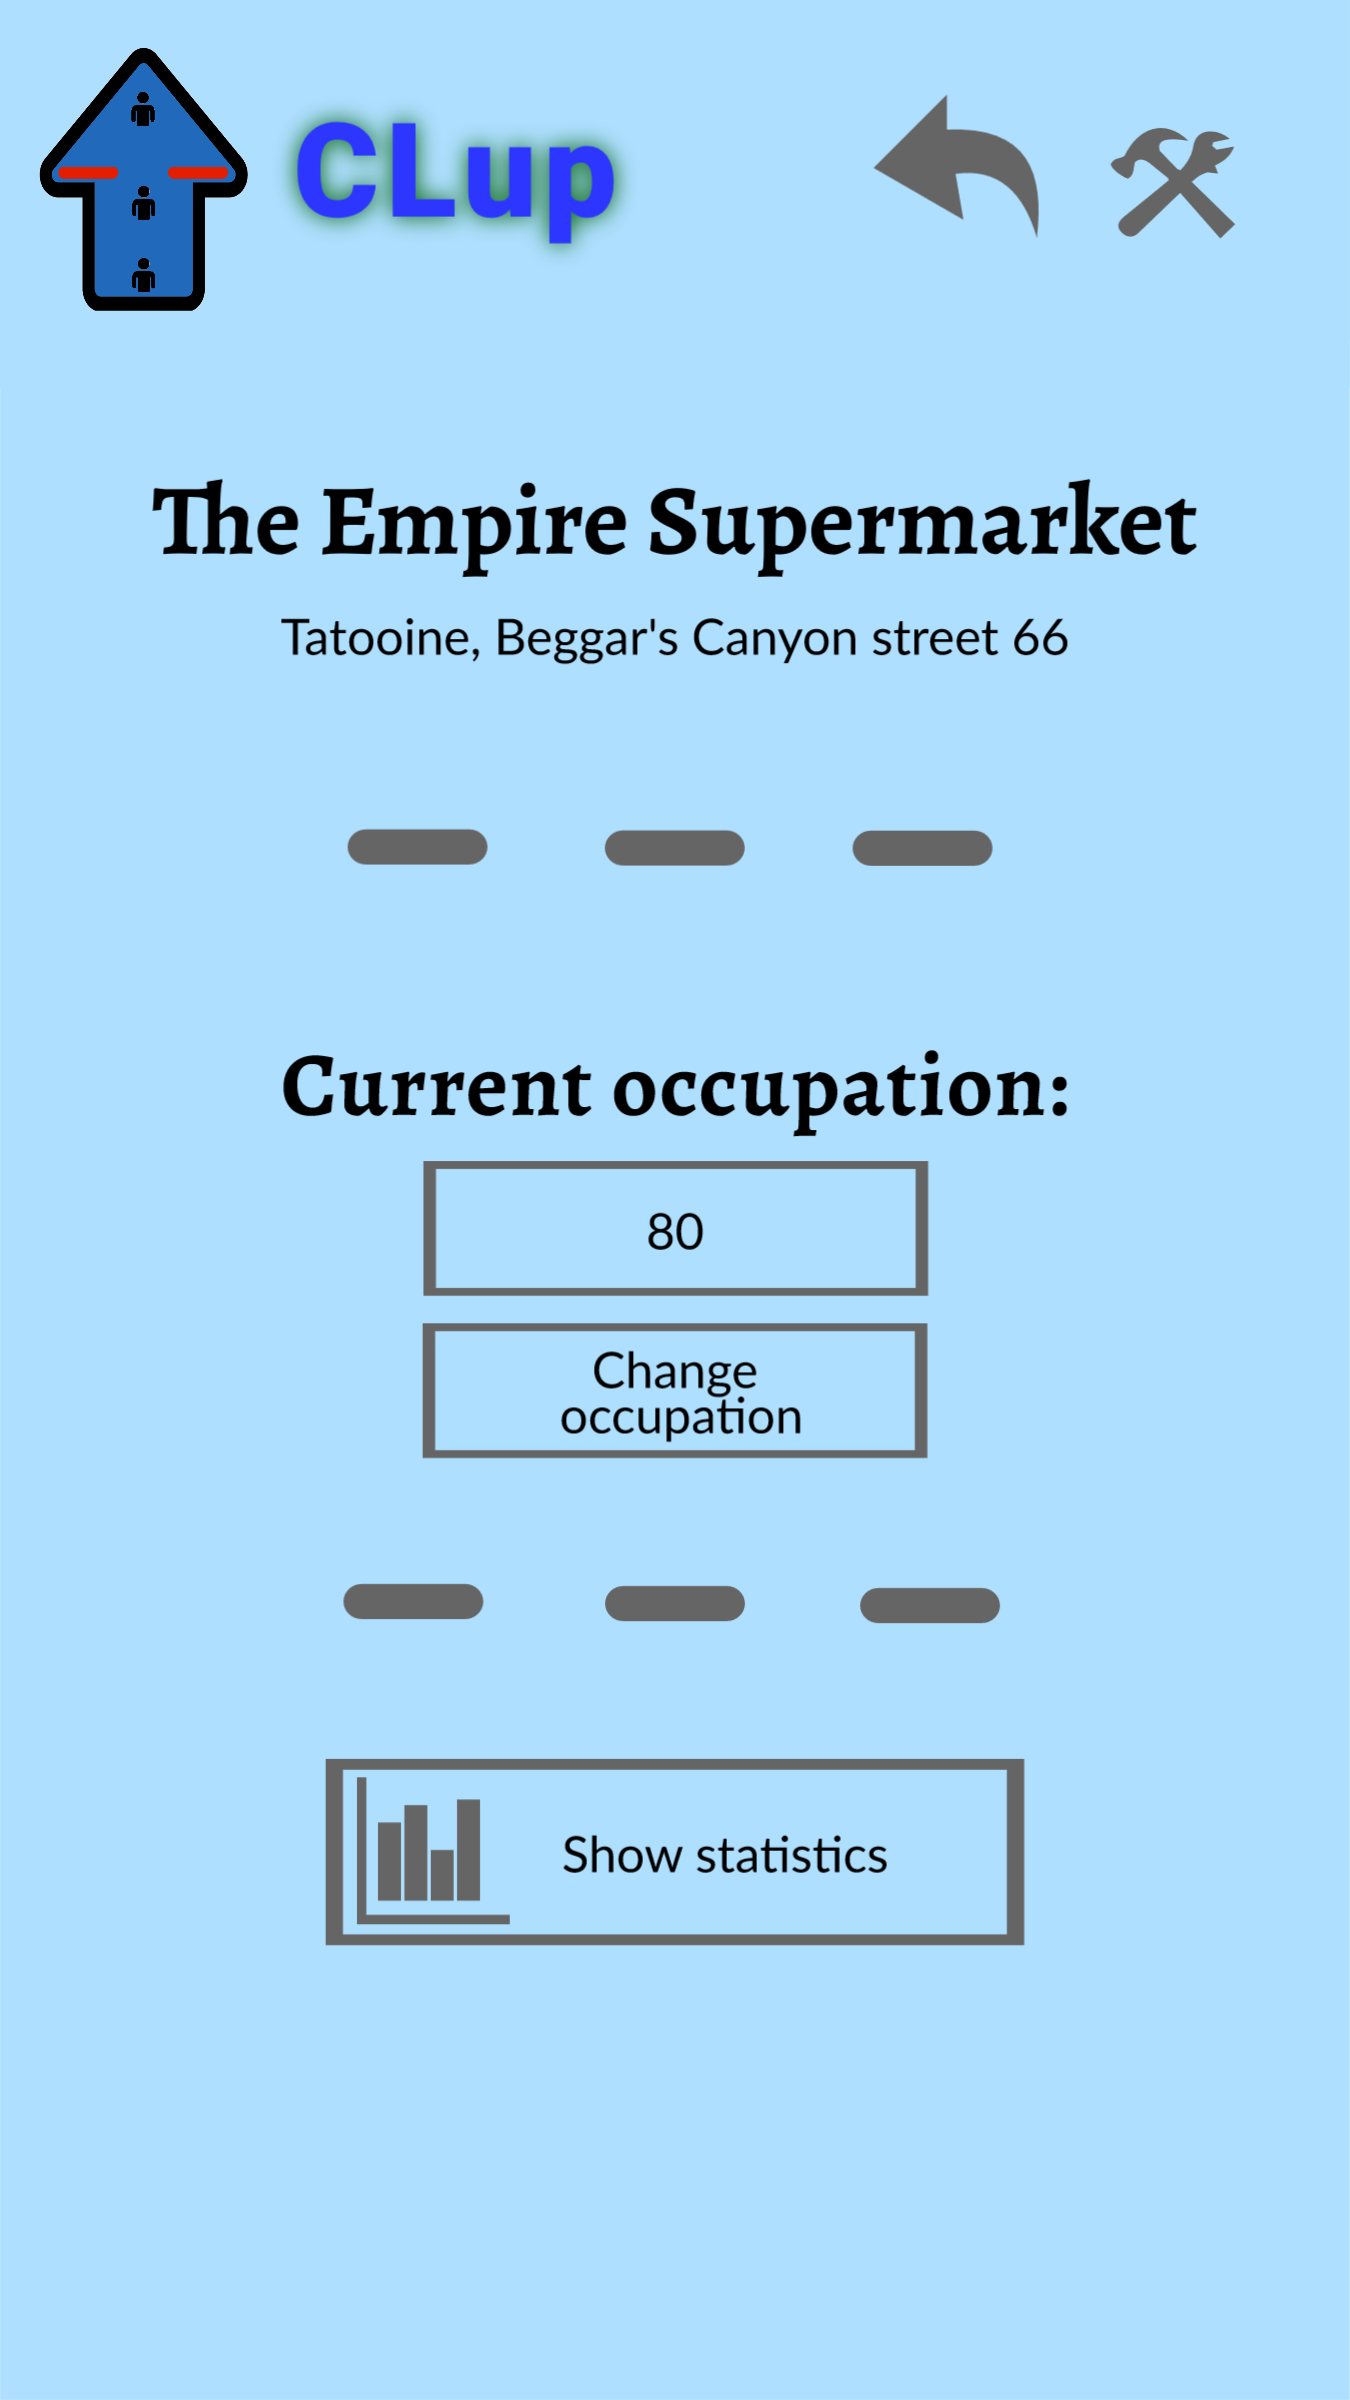
\includegraphics[scale=0.1]{Images/ModifyOccupation.png}
	\end{figure}
	
\end{itemize}
\subsubsection{Hardware interfaces}
The S2B requires the following hardware interfaces:
\begin{enumerate}
	\item {\bfseries Computer or smartphone}\\
	Users will need a computer or a smartphone to access the system's services which are provided via an application (only for smartphone owners) and a web application. Only users with an application will be able to receive notifications that alert them when it is time for them to depart and reach the store.
	\item {\bfseries Turnstiles}\\
	Turnstiles allow authorized customers to enter or exit the store by providing a means of identification. (i.e. QR, NFC)
	\item {\bfseries Ticket printer}\\
	The ticket printers located outside stores allows potential customers to queue up on premise provided that they identify themselves (e.g. social security card).
	\item \textbf{Monitor}\\
	A monitor located outside stores allows customers that queue up on premise to know when it is time for them to access the store.
\end{enumerate}

\subsubsection{Software interfaces}
The system uses a public API to locate the customer and provide him/her with notifications about the time he will need to depart to reach the store.

\subsubsection{Communication interfaces}
Customers can access the system through a working internet connection.

\subsection{Functional requirements}
\subsubsection{List of requirements}
\begin{enumerate}[label=R\arabic*]
	\item Turnstiles only unlock when activated by authorized customers.
	\item The number of customers in the store never exceeds the occupation set by the owner.
	%\item The customer is alerted when his/her turn is near.
	\item The monitor outside the store shows the number of the last authorized customer.
	\item The system allows customers and store owners to register and log in.
	\item The system must be able to validate the authenticity of the identifying information provided in registration requests.
	\item The system allows customers to search for a store among those registered by their owners.
	\item Registered customers can send a reservation request to the system.
	\item Registered customers can specify information about their visit (e.g. estimated duration, desired category of products).
	\item The system must use gathered data to build statistics. %TODO to ask.
	\item The system provides customers with means to verify that they are authorized.
\end{enumerate}
\subsubsection{Use cases}
%TODO: 'customer is notified' use case: is it useless?
\paragraph{Customer registration}
\begin{flushleft}
	\begin{tabular} { | m{3cm} | m{10cm} | }
		\hline
		Name & Customer registration\\
		\hline
		Actors & Customer\\
		\hline
		Entry condition & Customer has opened the smartphone application or the web app on his computer but has not logged in\\
		\hline
		Event flow & \begin{enumerate}
			\item a registration menu is provided to the customer
			\item from such menu the customer selects the option to sign up as customer
			\item the customer is then prompted to insert identifying information
			\item the customer inserts requested information
			\item the system validates provided information
			\item the system confirms the registration of the customer and saves information provided
		\end{enumerate}\\
		\hline
		Exit conditions & Customer has registered to the system\\
		\hline
		Exceptions & \begin{enumerate}
			\item a customer with same identifying information already exists
			\item validation of identifying information is not successful
			\item the customer decides to cancel the registration
		\end{enumerate}
		If one of the first two events described above occur, the application will alert the customer and provide him with the possibility to retry or go back to the initial menu.\newline If event 3 occurs the customer is redirected to the main page.\\
		\hline
	\end{tabular}
\end{flushleft}

\paragraph{Store owner registration}
\begin{flushleft}
	\begin{tabular} { | m{3cm} | m{10cm} | }
		\hline
		Name & Store owner registration\\
		\hline
		Actors & Store owner\\
		\hline
		Entry condition & Store owner has opened the smartphone application or the web app on his computer but has not logged in\\
		\hline
		Event flow & \begin{enumerate}
			\item a registration menu is provided to the store owner
			\item from such menu the store owner selects the option to sign up as store owner
			\item the store owner is then prompted to insert identifying information
			\item the store owner inserts requested information
			\item the system validates provided information
			\item the system confirms the registration of the store owner and saves information provided
		\end{enumerate}\\
		\hline
		Exit conditions & Store owner has registered to the system\\
		\hline
		Exceptions & \begin{enumerate}
			\item a store owner with same identifying information already exists
			\item validation of identifying information is not successful
			\item the store owner decides to cancel the registration
		\end{enumerate}
		If one of the first two events described above occur, the application will alert the store owner and provide him with the possibility to retry or go back to the initial menu.\newline If event 3 occurs the store owner is redirected to the main page.\\
		\hline
	\end{tabular}
\end{flushleft}

\paragraph{Customer queuing up remotely}
\begin{flushleft}
	\begin{tabular} { | m{3cm} | m{10cm} | }
		\hline
		Name & Customer queuing up remotely\\
		\hline
		Actors & Customer\\
		\hline
		Entry condition & Customer has logged in on the smartphone application or the web app on his computer\\
		\hline
		Event flow & \begin{enumerate}
			\item customer selects the option to queue up from main menu
			\item customer selects a store from the list of stores registered to the system
			\item customer selects to queue up
			\begin{itemize}
				\item with an immediate reservation
				\item with a future reservation (and optionally inserts desired categories of item he/she intends to buy and how much time he/she intends to spend at the store)
			\end{itemize}
			\item customer specify  whether he is going to reach the store by car or on foot
			\item customer submits reservation request
		\end{enumerate}\\
		\hline
		Exit conditions & Customer reservation is confirmed\\
		\hline
		Exceptions & \begin{enumerate}
			\item customer decides to cancel the reservation
		\end{enumerate}
	%TODO store e chiuso
		If one of the events described above occur, the application will alert the customer and provide him with the possibility to retry or go back to the initial menu\\
		\hline
	\end{tabular}
\end{flushleft}

\paragraph{Customer queuing up on premise}
\begin{flushleft}
	\begin{tabular} { | m{3cm} | m{10cm} | }
		\hline
		Name & Customer queuing on premise\\
		\hline
		Actors & Customer\\
		\hline
		Entry condition & Customer has reached the store ticket printer\\
		\hline
		Event flow & \begin{enumerate}
			\item customer selects the option to queue up from main menu of the ticket printer
			\item customer provides the ticket printer with a means of identification (e.g. social security card)
		\end{enumerate}\\
		\hline
		Exit conditions & Customer reservation is confirmed and a ticket is printed containing the following information:
		\begin{itemize}
			\item how much time he needs to wait before being able to enter the store
			\item a progressive number that will allow him to know when his/her turn is
		\end{itemize}\\
		\hline
		Exceptions & \begin{enumerate}
			\item customer decides to cancel the reservation
		\end{enumerate}
		If one of the events described above occur, the application will alert the customer and go back to the initial menu\\
		\hline
	\end{tabular}
\end{flushleft}

\paragraph{Customer entering store}
\begin{flushleft}
	\begin{tabular} { | m{3cm} | m{10cm} | }
		\hline
		Name & Customer entering store\\
		\hline
		Actors & Customer\\
		\hline
		Entry condition & Customer has logged in on the smartphone application and is at the entrance of a store\\
		\hline
		Event flow & \begin{enumerate}
			\item customer selects the option to show existing reservations from main menu of the phone app %TODO web app?????
			\item customer selects an existing reservation and if authorized (i.e. it is his turn to enter the store) he/she is given the means to identify him/herself (e.g. display QR or activate NFC)
			\item customer identifies him/herself at the turnstiles
		\end{enumerate}\\
		\hline
		Exit conditions & Customer enters the store\\
		\hline
		Exceptions & \begin{enumerate}
			\item customer is not authorized to enter the store
		\end{enumerate}
		If the event described above occurs, the turnstiles will not let the customer in\\
		\hline
	\end{tabular}
\end{flushleft}

\paragraph{Customer exiting store}
\begin{flushleft}
	\begin{tabular} { | m{3cm} | m{10cm} | }
		\hline
		Name & Customer exiting store\\
		\hline
		Actors & Customer\\
		\hline
		Entry condition & Customer has logged in on the smartphone application and is in a store\\
		\hline
		Event flow & \begin{enumerate}
			\item customer selects the option to show existing reservations from main menu
			\item customer selects an existing reservation and if authorized (i.e. it is his turn to enter the store) he/she is given the means to identify him/herself (e.g. display QR or activate NFC)
			\item customer identifies him/herself at the turnstiles
		\end{enumerate}\\
		\hline
		Exit conditions & Customer exits the store\\
		\hline
		Exceptions & \\
		\hline
	\end{tabular}
\end{flushleft}

\paragraph{Store owner registering a store}
\begin{flushleft}
	\begin{tabular} { | m{3cm} | m{10cm} | }
		\hline
		Name & Store owner registering a store\\
		\hline
		Actors & Store owner\\
		\hline
		Entry condition & Store owner has logged in on the smartphone application or the web app on his computer\\
		\hline
		Event flow & \begin{enumerate}
			\item store owner selects the option register a store from main menu
			\item store owner inserts necessary information and sets up equipment (i.e. connect printer, monitor and turnstiles to the system)
			\item store owner submits store registration request
		\end{enumerate}\\
		\hline
		Exit conditions & Store registration is confirmed\\
		\hline
		Exceptions & \begin{enumerate}
			\item information is missing or incorrect
			\item equipment is not working properly			\item store owner decides to cancel the store registration
		\end{enumerate}
		If one of the events described above occur, the application will alert the store owner and provide him with the possibility to retry or go back to the initial menu\\
		\hline
	\end{tabular}
\end{flushleft}

\paragraph{Store owner setting maximum occupation of one of his stores}
\begin{flushleft}
	\begin{tabular} { | m{3cm} | m{10cm} | }
		\hline
		Name & Store owner setting maximum occupation of one of his stores\\
		\hline
		Actors & Store owner\\
		\hline
		Entry condition & Store owner has logged in on the smartphone application or the web app on his computer\\
		\hline
		Event flow & \begin{enumerate}
			\item store owner selects one of his stores from the list reachable form the main menu
			\item store owner views current occupation of his store, and current occupation threshold
			\item sets the new desired occupation threshold
		\end{enumerate}\\
		\hline
		Exit conditions & The new occupation threshold is set\\
		\hline
		Exceptions & \begin{enumerate}
			\item the threshold value is inadequate
		\end{enumerate}
		If the event described above occurs, the application will alert the store owner and provide him with the possibility to retry or go back to the initial menu\\
		\hline
	\end{tabular}
\end{flushleft}